\documentclass[12pt]{report}
\usepackage{amsmath, amssymb, amscd, amsthm, amsfonts}
\usepackage{bookmark}
\usepackage[utf8]{inputenc}
\usepackage{graphicx}
% \usepackage[hyphens]{url}
\usepackage{hyperref}
\usepackage{float}
\usepackage{pgf}
\usepackage{xcolor}
\usepackage{tikz}
\usepackage{titlesec}
\usepackage{mdframed}
\usepackage[shortlabels]{enumitem}
\usepackage{indentfirst}
\usepackage{float}
\usepackage[vertfit]{breakurl}
\usepackage{graphicx}
\usepackage{subfig}
\usepackage{booktabs}
\usepackage{xltabular}
\usepackage[backend=biber]{biblatex} 
\addbibresource{references.bib}


\usepackage{geometry}
 \geometry{
 a4paper,
 total={170mm,257mm},
 left=20mm,
 top=20mm,
 }

 \linespread{1.5}


\usepackage{fancyhdr}
\pagestyle{fancy}
\fancyhf{}
\rhead{\textbf{Cody Riley}}
\lhead{\textbf{Mathematics Project}}
\rfoot{Page \thepage}

\title{Solving Dynamical Systems in Python}
\author{Cody Riley}
\date{8/10/2022}

\begin{document}
\maketitle
\newpage
\chapter{The Development Phase}
\section{Stages of Development}
The development process of my dynamical system solver was relatively straightforward in the early stages of development. The first stage of development was to build a solid plan for what I planned to make. As discussed in my statement of intent, I wanted to develop an easy-to-use piece of software that would allow any user to input a set of first-order differential equations and have the python script approximate a solution to the corresponding dynamical system. In the early stages of planning, I thought it would be good to allow the user to input how many equations they would like to include in the solver. However, although the final build allows this to occur, it is more likely for bugs to occur, and the app becomes very tedious to use.
\smallskip

At first, I thought building such a program would be relatively straightforward, and I assumed I would have no issues. However, it proved more difficult than I anticipated, as I had to ensure that the correct number of equations were being generated alongside the number of variables. The name of the variables was also a challenge, and for simplicity, during the early stages of development, I decided to use the variable naming convention of $x_{n}$, where $n \in \mathbb{Z}^{+}$.
\section{Positive Outcomes}
There were many positive outcomes in the development of my Dynamical Systems app. Firstly, I successfully allowed users to enter a system of $n$ equations in the terminal version of the application.
\section{Challenging Parts of Development}
Handling discontinuities of functions a user inputs was one of the biggest challenges in the development of the Python application. For example, say you had a simple one-dimensional problem, equivalent to
\begin{equation*}
    \frac{dy}{dt} = \frac{1}{t} 
\end{equation*}
over a timespan of $[-5,5]$ (this is just the domain we will plot over). In this case, we would encounter an error because our solver cannot solve the differential equation for $t > 0$ and hence we are unable to plot an accurate solution to that part of the solution.
\section{Future Developments for the Project}
I plan to work on this project further past the deadline. I just like to have projects to do in my spare time, and there are a few features I will be adding to my project. Firstly, I would like to add some functionality that I ran out of time to add. The plan was to give the user the option to add as many equations as they would like to solve the dynamical system. This would result in a much more complex system being solved. This functionality works in the terminal version of the program, however, I just ran out of time to give the GUI the ability to change how many equations the algorithm had to solve. I would also like to add the ability for the user to clear the current plot showing on the GUI, as this would result in better accessibility to the overall use of the tool. For example, at the moment, the current build of the Dynamical Systems Solver App only allows for you to plot a single graph on the canvas, and after plotting this graph you would have to restart the app to plot the next one. I have tried a few approaches to this problem already,
\chapter{How to Use the Application}
As mentioned in the development process of the program, there are two different versions of the program that has been developed. One version uses the terminal and has more capability, and the other version takes advantage of a GUI but currently has less functionality.
\smallskip

The first version we will discuss is the version involving only the terminal. The first instruction that a user is prompted with is how many equations they would like to enter. There is no limit to the number of equations a user can enter, however, it is highly recommended that at maximum three equations are entered. Next, the user will be prompted to enter a lower bound $t_{min}$ which is required to be a float. After successfully entering a lower bound, the user will be prompted to enter an upper bound $t_{max}$ which requires the same conditions as $t_{min}$.
\smallskip

The user will then be prompted with a statement saying that they are solving a dynamical system with $n$ equations, where $n$ is the number entered in the first prompt. In the same statement, the variables generated will be defined. This has the form of a vector $x = (t,x_{1},\cdots, x_{n})$. For example, if we were to enter $n = 2$, then the variables are defined to be $x = (t,x_{1},x_{2})$ where $t$ is the time component. Next, the user will be asked to define their equations in-terms of the variables that have been defined. In mathematical terms, this is denoted as $f_{n}(x)$. After the user has entered all the equations, then the user will be prompted to enter initial conditions for all the solutions. These initial conditions are defined to occur at $t_{0} = t_{min}$. For example, if $t_{min} = -5$, then $x_{n}\left(t_{min}\right) = \alpha_{n}$.
\smallskip

The final step that we need to take is to enter the number of steps we wish to use to numerically approximate a solution to the dynamical system. This will then be used to split our time span into $k$ sub intervals. 
\section*{Example Calculation}
We will consider a basic example for our calculation. We will consider the case where the number of equations we enter is $n = 2$. The timespan that we will be considering is $\mathbb{T} = [-5,5]$ which means the lower bound is $-5$ and the upper bound is $5$. We will then enter our equations which will be 
\begin{equation*}
    \begin{split}
        \frac{dx_{1}}{dt} &= 1 - x_{1} + x_{2} \\
        \frac{dx_{2}}{dt} &= x_{1} - x_{2}
    \end{split}
\end{equation*}

\section*{GUI Version}
The graphical user interface version of the dynamical system solver application is much more accessible and easier to use compared to the terminal version. Throughout this section of my report, I will explain how to use the GUI version of my project with a worked example.
\begin{figure}[H]
    \centering
    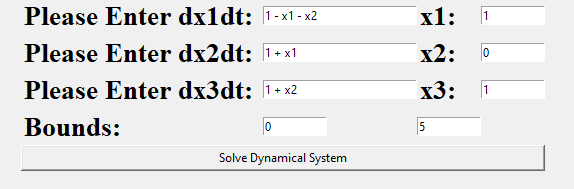
\includegraphics[scale = 0.8]{demo 1.png}
    \caption{Image showing the input fields for the Dynamical Systems solver and the execute button.}
\end{figure}
In the GUI, we can see that we have entered three equations, three initial conditions, and the bounds. These fields are strictly required, otherwise the python script that handles all the technical calculations require all the pieces of information. The equations that we input into the fields adjacent to the label 'Please Enter $dx_{n}dt$' are required to use only the variables $t$, $x_{1}$, $x_{2}$, and $x_{3}$. If any other variables are detected that are not defined, then the calculation will cease and an error will be displayed in the terminal. 
\begin{figure}[H]
    \centering
    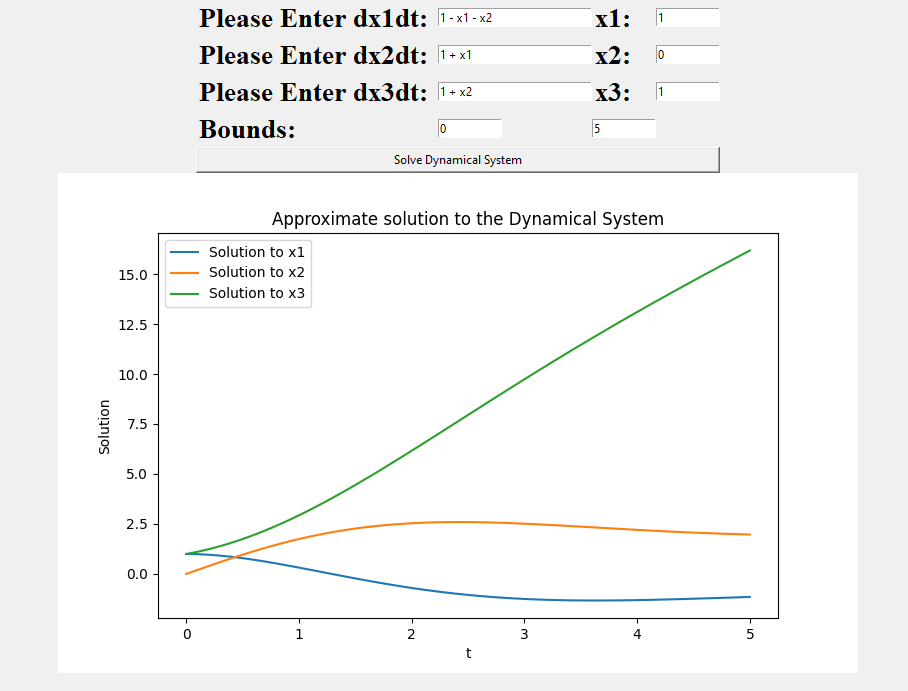
\includegraphics[scale = 0.7]{demo 2.png}
    \caption{Image showing the input fields for the Dynamical Systems solver and the execute button. It also shows the numerically approximated solutions to the differential equations.}
\end{figure}



\end{document}